% !TeX encoding = UTF-8
\chapter*{ВВЕДЕНИЕ}
\addcontentsline{toc}{chapter}{ВВЕДЕНИЕ}

Основная цель данного руководства состоит в объяснении пользователям основных
возможностей \TeX овского класса {\itshape thesisby} версии 1.1 для  оформления
диссертаций в соответствии с инструкцией  от 24 декабря 1997~г. \textnumero ~178 с
изменениями и дополнениями \textnumero 7/603 от 09.03.2006~г., \textnumero 7/743 от
03.09.2007~г. и \textnumero 3 от 28.02.2014 г. действующей в Республике Беларусь. В руководстве даны основные рекомендации, которым нужно следовать для того, чтобы диссертация соответствовала необходимым требованиям. Также приведен ряд указаний, который может существенно упростить подготовку диссертации. В данном руководстве предполагается первоначальное знакомство пользователя с \TeX ом, а также умение пользоваться основными его возможностями.

Официальный сайт проекта:
\href{https://github.com/belgraviton/thesisby}{https://github.com/belgraviton/thesisby}

Поддержка данного класса осуществляется в следующем сообществе:
\href{http://community.livejournal.com/thesisby/}{
http://community.livejournal.com/thesisby/}

Электронный адрес основного разработчика: thesisby@tut.by

Следует заметить, что данное руководство оформлено с использованием описываемого класса {\itshape thesisby}. Поэтому у пользователей есть непосредственная возможность визуального знакомства с возможностями данного класса. Наряду с самим классом на официальном сайте проекта можно скачать \TeX код данного руководства, который может быть использован как шаблон для диссертации. Кроме данного простого шаблона для диссертации может оказаться удобным использовать сцепленные шаблоны для диссертации, автореферата и презентации, которые также могут быть найдены на сайте. Более подробная информация про данные шаблоны представлена в Приложении~\ref{app:template}.

Для создания данного класса был использован исходный код класса {\itshape
dissert.cls} (автор: Андрей Мартовлос), который был доработан для удовлетворения
необходимым требованиям. Также часть кода была взята из класса {\itshape G7-32}
(автор: Алексей Томин). 

Так как исходный класс {\itshape dissert.cls} был создан из класса {\itshape report.cls} и  стилевого файла {\itshape size14.clo}, которые распространяются по \href{http://www.latex-project.org/lppl/}{общественной лицензии проекта Латех (LaTeX Project Public License, LPPL)}, следовательно класс {\itshape thesisby} также подлежит действию данной лицензии.

Данный программный продукт является свободным программным обеспечением. Вы вправе распространять его и/или модифицировать в соответствии с условиями версии 1.3c либо по вашему выбору с условиями более поздней версии общественной лицензии проекта Латех.


\newpage
{\large \bfseries История версий:}
\begin{itemize}
 \item 0.8 (30 марта 2008 г.) - Начальная версия, созданная на основе класса {\itshape
dissert.cls} (автор: Андрей Мартовлос).
 \item 0.82 (8 декабря 2008 г.):
\begin{itemize}
 \item Внесены исправления в реализацию окружения для заметок к формулам
(\verb|eqrem|).
 \item Поддержка русского языка для стандартных названий включена, как опция
класса, по умолчанию.
 \item Реализовано автоматическое подключение расширения к пакету
\verb|longtable|. Теперь не требуется включать файл {\itshape longtabledef.tex}
в документ командой \verb|\include|. Файл {\itshape longtabledef.tex} исключен
из набора для класса.
 \item Реализована совместимость класса с пакетом \verb|hyperref|(см.
Главу~\ref{chap:draft}).
\end{itemize}
 \item 0.9 (15 мая 2009 г.):
\begin{itemize}
 \item Внесены исправления в оформление списка литературы.
 \item Реализована возможность использования класса для оформления научных
отчетов по ГОСТу 7.32-2001 (устарело, рекомендуется использовать класс {\itshape repgost} \cite{repgost}).
 \item Внесены исправления в реализацию окружения для заметок к формулам
(\verb|eqrem|).
\end{itemize}

 \item 1.0 (15 июля 2012 г.):
\begin{itemize}
	\item Удалена точка в оглавлении после номера главы.
	\item Проведено более трех лет апробации класса.
\end{itemize}

 \item 1.1 (1 сентября 2016 г.):
\begin{itemize}
	\item Стиль приведен в соответствие с требованиями правил 2014 г.(нумерация страниц сверху и точка после нумерации иллюстраций, Nick Petrovsky).
	\item Расширение возможностей окружения \verb|\eqrem| (возможность переноса части окружения на следующую страницу, Vladzimir Leszkiewicz, см. уравнение \ref{eq:H0}).
\end{itemize}

\item 1.2 (30 июля 2020 г.)
\begin{itemize}
	\item (TBD)~Шаблон переведен в кодировку UTF-8. Реализована базовая поддержка XeLaTeX, режим совместимости с PDFLatex сохранен.
	\item (TBD)~Библиографический список поддерживает UTF-8.
	\item (TBD)~Добавлено руководство по использованию в системах Overleaf и ShareLatex
\end{itemize}

\end{itemize}



\newpage
\chapter{НАЧАЛО ДИССЕРТАЦИИ}

\section{Преамбула}

Класс {\itshape thesisby} реализуется посредством файла {\itshape thesisby.cls}.
Выбор класса {\itshape thesisby} для оформления документа осуществляется путем 
задания первой строкой в преамбуле декларации \verb|\documentclass{thesisby}|,
где по умолчанию устанавливается русский язык для стандартных названий глав и
разделов. Для использования белорусских названий следует задать опцию {\itshape
bel} в квадратных скобках перед названием класса. При работе с классом файл {\itshape
thesisby.cls} должен находится в одной папке с \TeX овским документом,
использующим данный класс.

Также в преамбуле может понадобиться подключить ряд пакетов: {\itshape inputenc}
(кодировка), {\itshape babel} (поддержка языков), {\itshape graphicx} (работа с
графикой), {\itshape array} (широкие возможности работы с таблицами), {\itshape
longtable} (работа с таблицами, занимающими несколько страниц), {\itshape
amsmath, amssymb, amsfonts} (математические пакеты). Все главы, разделы и
подразделы в документе печатаются с абзацным отступом, поэтому при работе с
классом не требуется подключение пакета {\itshape indentfirst}.

\section{Титульный лист, оглавление и ненумеруемые части диссертации}

Титульный лист оформляется в окружении \verb|titlepage| с использованием стандартных окружений \verb|center| (для центрирования) и  \verb|tabbing|(для создания текста упорядоченного по колонкам), команд для позиционирования \verb|\hspace|, \verb|\vspace|, \verb|\bigskip, \medskip, \smallskip| и деклараций для управления характеристиками шрифта \verb|\large, \bfseries|.

Оформление оглавления обеспечивается включением в документ команды
\verb|\tableofcontents| и правильной передачей названий ненумеруемых глав и
разделов (таких как введение, общая характеристика работы и заключение)
посредством команды \verb|\addcontentsline{toc}{Тип секции}{Название секции}|,
где второй аргумент указывает тип части, например chapter или section, а
последний ее название. При этом сами части начинаются заданием команд
секционирования со звездочками, например \verb|\chapter*{Название секции}|.

\newpage
\chapter{СТАНДАРТНЫЕ ВОЗМОЖНОСТИ КЛАССА}

\section{Главы, разделы, подразделы и пункты}

Главы печатаются командой \verb|\chapter{Название главы}|, разделы и подразделы
\verb|\section{Название раздела}| и \verb|\subsection{Название подраздела}|
соответственно, а пункты, в свою очередь, задаются командой
\verb|\subsubsection{Название пункта}|. Пункт может не иметь заголовка.

\subsection{Пример подраздела}

\subsubsection{Пример пункта}

Текст пункта.

\subsubsection{} Пример пункта без заголовка. Пример пункта без заголовка. Пример пункта без заголовка. Пример пункта без заголовка. Пример пункта без заголовка. Пример пункта без заголовка. Пример пункта без заголовка. Пример пункта без заголовка.


\section{Нумерация страниц}

В связи с требованиями дополнения \textnumero 3 от 28.02.2014 г к правилам оформления диссертации нумерация страниц осуществляется сверху. Для регулирования отступа номера от верха текста можно использовать команду: \verb|\headsep = 3mm| в преамбуле.

Управление верхним и нижним колонтитулом осуществляется с помощью пакета {\itshape fancyhdr}. Например, номера страниц можно переместить вниз страницы следующими командами в преамбуле:

\verb|\fancyhead{}|

\verb|\fancyfoot[C]{\thepage}|

\section{Формулы и уравнения}

Для оформления формул и уравнений используются стандартные возможности \LaTeXe.
Их нумерация осуществляется автоматически в пределах главы, как это
продемонстрировано для формул (\ref{eq:H0}) и (\ref{eq:Hmn}).

Для пояснения значений символов и числовых коэффициентов, входящих в формулу или
уравнение используется специальное окружение \verb|eqrem|, в котором значения
символов и коэффициентов отделяются одно от другого двумя последовательными
командами~\verb|\\| и \verb|&|.

Ниже приведен простейший пример
\begin{equation}\label{eq:H0}
H_0 = \frac{p^2}{2 m} + a_0\, x^4 - a_2\, x^2 + l\, x - \gamma \tau,
\end{equation}
\begin{eqrem}
$p$ -- импульс частицы,\\
& $m$ -- масса частицы,\\
& $x$ -- координата частицы,\\
& $a_0, a_2$ -- параметры системы\\
& $l$ -- коэффициент трения\\
& $\gamma$ -- параметр сдерживания\\
& $\tau$ -- усиление параметра сдерживания.
\end{eqrem}

А это уже более сложный пример
\begin{align}
H^0_{m\, n} & = \delta_{m + 4 \; n} \;\frac{a_0 g^2}{4} \sqrt{(m + 1)(m + 2)(m +
3)(m +
4)} \notag\\
 & + \delta_{m + 2 \; n} \;\frac{g}{2} a_0  (2 m + 3) \sqrt{(m
+ 1)(m  + 2)}.\label{eq:Hmn}
\end{align}
\begin{eqrem}
$g = \frac{m}{a_0}$ -- числовой коэффициент.
\end{eqrem}


\section{Графики}

Ниже приведен рисунок \ref{fig}, который оформлен в соответствии с требованиями
для диссертаций.

\begin{figure}[h!]
\begin{center}
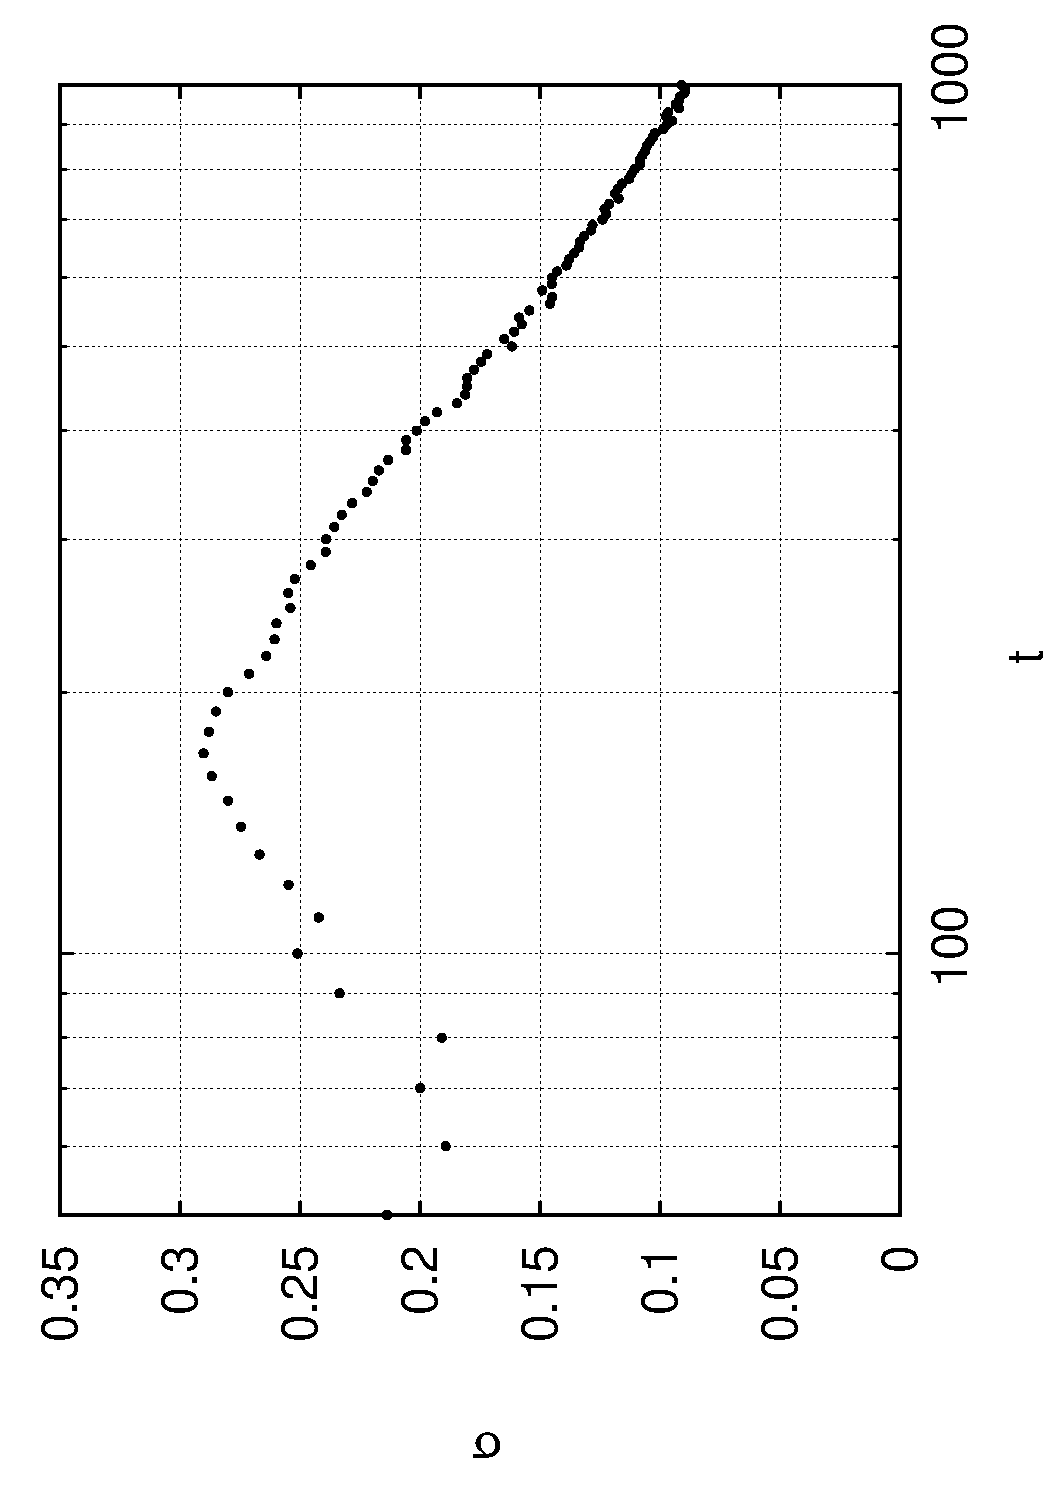
\includegraphics[angle=270,width=10cm]{test}\\[2mm]
{\small Подрисуночный текст. Подрисуночный текст}
\caption{Подпись к рисунку. Дополнительная информация}\label{fig}
\end{center}
\end{figure}

Рисунок оформляется с использованием стандартного окружения \verb|figure|,
который обеспечивает его автоматическую нумерацию. Рисунок и подпись вставляются
при помощи стандартных команд \verb|\includegraphics| и
\verb|\caption{Подпись}| соответственно, а подрисуночный текст путем добавления
после команды \verb|\includegraphics| с новой строки текста записанного с декларацией \verb|\small|. Для
того, чтобы увеличить отступ между рисунком и подрисуночным текстом можно после
команды вставки рисунка (\verb|\includegraphics|) воспользоваться командой
перехода на новую строку со вставкой дополнительного вертикального отступа
\verb|\\[len]|, где \verb|len|--  высота дополнительного отступа.


\section{Работа с таблицами}

\subsection{Простые таблицы}

Для создания таблиц используется окружение \verb|table|, которое обеспечивает
нумерацию и создание заголовка. Для помещения заголовка над таблицей в начале
указанного окружения необходимо задать команду \verb|\capition{Подпись}|. Сама
таблица может оформляться с помощью стандартного окружения \verb|tabular|.
Пример таблицы приведен ниже (таблица \ref{tab:1}, см. исходный код).

\begin{table}[h]
\caption{Характеристики процессов формирования волокон из гидратцеллюлозы}
\label{tab:1}
\begin{center}
\begin{tabular}{|l|c|c|}
\hline
Наименование показателей & Вискоза & Камилон \\
\hline
Максимальная фильерная вытяжка, \% &12 &80\\
\hline
Температура осадительной ванны, \si{\celsius} &50 &20\\
\hline
Максимальная кратность вытягивания, \% &100 &30\\
\hline
\end{tabular}
\end{center}
\end{table}

В диссертации для таблиц допускается использование шрифта, который на 1-2 пункта
меньше, чем в остальном тексте. Для реализации данной возможности необходимо
подключить пакет {\itshape array} и поместить команду \verb|>{\small}| перед
указателями для колонок в аргументе окружения \verb|tabular|. Пример
использования данной команды для шапки таблицы \ref{tab:2} следующий:
\verb@\begin{tabular}{|>{\small}l|>{\small}c|>{\small}c|}@.

\begin{table}[h]
\caption{Приведенная выше таблица с шрифтом уменьшенным на 2 пункта}
\label{tab:2}
\begin{center}
\begin{tabular}{|>{\small}l|>{\small}c|>{\small}c|}
\hline
Наименование показателей & Вискоза & Камилон \\
\hline
Максимальная фильерная вытяжка, \% &12 &80\\
\hline
Температура осадительной ванны, \si{\celsius} &50 &20\\
\hline
Максимальная кратность вытягивания, \% &100 &30\\
\hline
\end{tabular}
\end{center}
\end{table}

\subsection{Таблицы с больш\'{и}м количеством строк}
\label{sec:ltable}

Перенос таблиц с большим количеством строк на следующий лист удобно реализовать
с помощью окружения \verb|longtable|, которое используется вместо окружения
\verb|table| и требует подключения пакета {\itshape longtable}. В приложении
\ref{app:table} приведен пример такой таблицы.

Для правильного оформления заголовка и подписей к таблице необходимо использовать команды \verb|\endfirsthead, \endhead, \endfoot,\endlastfoot| (см. \cite[раздел 12.5]{Kotelnikov}). Заголовок над первой частью таблицы указывается с использованием стандартной команды \verb|\caption{Подпись}|, которая задается перед командой \verb|\endfirsthead|. Над другими частями таблицы должно быть написано ``Продолжение таблицы'' с соответствующим номером. Для реализации этого требования необходимо перед командой \verb|\endhead| кроме описания заголовка таблицы записать \verb|\multicolumn{ncols}{l}{Продолжение таблицы \ref{tableref}}|, где {\itshape ncols}-- число колонок в таблице, {\itshape tableref} -- метка для таблицы, которую нужно задать в начале окружения \verb|longtable| командой \verb|\label{tableref}| (см. исходный код для приложения \ref{app:table}).

\subsection{Таблицы с больш\'{и}м количеством столбцов}
\label{sec:gtable}

Таблица с большим количеством столбцов, согласно правилам, может быть разбита на
части  и помещена в пределах страницы одна часть над другой. Данную возможность
можно реализовать используя стандартные средства \LaTeXe{}  и окружение
\verb|table|. Для этого каждая отдельная часть таблицы оформляется с
использованием окружения \verb|tabular|. Над первой частью пишется заглавие
(используется \verb|\caption{Подпись}|), а остальные части отделяются небольшим
вертикальным отступом \verb|\smallskip| или \verb|\medskip| и подписываются
согласно требованиям. Пример такой таблицы приведен в
приложении~\ref{app:gtable}.

\section{Примечания}

В данном классе существует возможность оформления примечаний при помощи
окружений \verb|comments| и \verb|comment|. В первом предполагается наличие
нескольких примечаний, которые нумеруются командой \verb|\item|, а второе
предназначено для включения в текст одиночного примечания без нумерации. Сначала
приведем пример окружения \verb|comments|:

\begin{comments}
\item Текст первого абзаца первого примечания. Текст первого абзаца первого
примечания. Текст первого абзаца первого примечания. Текст первого абзаца
первого примечания. Текст первого абзаца первого примечания.

Текст второго абзаца первого примечания. Текст второго абзаца первого
примечания. Текст второго абзаца первого примечания. Текст второго абзаца
первого примечания.

\item Текст второго примечания. Текст второго примечания. Текст второго
примечания. Текст второго примечания.
\end{comments}

А теперь окружения \verb|comment|:
\begin{comment}
Текст примечания. Текст примечания. Текст примечания. Текст примечания. Текст
примечания. Текст примечания. Текст примечания. Текст примечания. Текст
примечания. Текст примечания. Текст примечания. Текст примечания.

Текст примечания. Текст примечания. Текст примечания. Текст примечания. Текст
примечания. Текст примечания. Текст примечания. Текст примечания. Текст
примечания. Текст примечания. Текст примечания. Текст примечания. Текст
примечания. Текст примечания. Текст примечания.
\end{comment}

По приведенным двум примерам видны отличия в оформлении упомянутых двух
окружений.


\chapter{ОФОРМЛЕНИЕ БИБЛИОГРАФИИ}

В рассматриваемом классе используется стандартное окружение
\verb|thebibliography| для оформления списка использованных источников и
аналогичное ему окружение \verb|mybibliography| для списка публикаций
соискателя. С обоими окружениями принципы работы одинаковы. Сами окружения
оформляются с использованием команды создания библиографической записи
\verb|\bibitem{метка}|, а ссылки в тексте формируются с использованием
стандартной команды \verb|\cite{метка}| или ее расширенной формы
\verb|\cite[текст]{метка}|, если необходимо указать дополнительную информацию
для данного источника.

Приведем несколько примеров ссылок. Простые ссылки на использованные источники
\cite{Kotelnikov,article} и 
\cite{proc}. Более сложные имеют следующий вид \cite[с. 25]{Kotelnikov} и
\cite[формула 2]{article}. А теперь ссылки на англоязычные работы соискателя
\cite{myarticle,myproc}  и на русскоязычные работы в более сложном виде
\cite[формула~4]{myrussianarticle} и \cite[глава~2]{mybook}.

Так же следует обратить внимание на то, что, в случае необходимости оформления
списка литературы по ГОСТу 7.1—2003 \cite{gost7-1}, удобно пользоваться программой для создания библиографии BiBTeX (см. \cite[глава 13]{Kotelnikov}). Существуют специальные
библиографические стилевые файлы, которые позволяют оформлять список литературы
с результатами близкими к установленным требованиям. Это стили {\itshape
gost71s2003.bst} и {\itshape gost71u2003.bst} соответственно, с сортировкой и без
нее. Данные стили представлены на сайте проекта {\itshape thesisby}~\cite{gost71_2003}.

Для использования указанных стилей в записи  библиографической базы
данных, использующей русский язык, необходимо добавить строку
\verb|language = {russian}|, а в случае использования сортировки для англоязычных изданий также нужно обязательно включить опцию \verb|language = {english}|.


\chapter{ДОПОЛНИТЕЛЬНЫЕ ВОЗМОЖНОСТИ КЛАССА}

\section{Черновой режим работы над диссертацией}
\label{chap:draft}

Существует ряд пакетов, которые предназначены для более удобной организации
работы над документами в \LaTeXe{} в черновом режиме. В данном разделе пойдет
речь о двух  таких пакетах: {\itshape hyperref} и {\itshape refcheck}. Первый
предназначен для включения гиперссылок в документ, второй для поиска в нем
неиспользуемых и бесполезных ссылок.

В пакете {\itshape hyperref} реализована поддержка гиперссылок и закладок, что является очень удобным средством для быстрой навигации по документу \cite{hyperref}. Данный пакет подключается командой \verb|\usepackage[список опций]{hyperref}| в преамбуле документа. Опции также можно задать при помощи команды \verb|\hypersetup{список опций}|. Среди опций следует отметить {\itshape unicode}, которая требуется для отображения кириллических букв в закладках pdf-документа, {\itshape colorlinks}, для выделения ссылок различными цветами, и {\itshape pagebackref} либо {\itshape  backref}, которые предназначены для создания «обратных» гиперссылок в библиографическом списке: в конец каждого элемента списка в виде гиперссылок добавляются номера страниц (опция {\itshape pagebackref}) или номера разделов (опция {\itshape backref}), где встречаются «прямые» ссылки на этот элемент. К сожалению, обратные гиперссылки не включаются в список публикаций соискателя.

Данное руководство пользователя было получено с использованием 
компилятора pdf\LaTeX{} при подключении пакета {\itshape hyperref} с опциями {\itshape unicode},  {\itshape colorlinks} и {\itshape pagebackref}. Более подробную информацию можно получить в специальной литературе по данному пакету \cite{hyperref,hyperrefop}.

Пакет {\itshape refcheck} предназначен для поиска в документе непронумерованныx уравнений и неиспользуемых библиографических ссылок. Для этой цели на полях документа автоматически размещаются имена меток, которые помечаются знаками вопроса в случае их неиспользованности. К сожалению, следует заметить, что данный пакет при работе с классом {\itshape thesisby} обрабатывает только список использованных источников. Для использования пакета следует подключить его в преамбуле документа следующей командой: \verb|\usepackage{refcheck}|. Для совместной работы с {\itshape hyperref}, {\itshape refcheck} должен загружаться после него. Дополнительную информацию по пакету следует искать в специальной литературе, например \cite{refcheck}.


\section{Оформление отчетов с помощью пакета {\itshape thesisby} (устарело)}\label{sec:rep}

Начиная с версии 0.9 класс {\itshape thesisby} мог использоваться для оформления отчетов. Для этого нужно было задать опцию {\itshape rep} в декларации класса в преамбуле документа. Однако, как показал опыт, {\itshape thesisby} не полностью соответствует ГОСТу 7.32-2001 \cite{gost7-32}. В частности, отличия наблюдаются в оформлении подписей к рисункам и названий приложений. Поэтому на основании {\itshape thesisby} был создан класс {\itshape repgost}, который соответствует требуемому ГОСТу~\cite{repgost}. Класс {\itshape thesisby} по прежнему для совместимости имеет опцию {\itshape rep}, однако, использовать класс для оформления отчетов \underline{не рекомендуется}.

В отличие от диссертации основной единицей секционирования в документе является раздел (\verb|\section|), а не глава (\verb|\chapter|). Но для приложений по прежнему используется команда \verb|\chapter|. Особенности оформления отчетов также касаются оформления списка исполнителей и нумерации формул, о которых рассказывается в следующих подразделах.

\section{Оформление отчетов с помощью пакета {\itshape repgost}}\label{sec:repgost}

Для удовлетворения ГОСТу 7.32-2001 на основании класса {\itshape thesisby} был создан класс {\itshape repgost}. В нем присутсвуют существенные отличия. Основным разделом секционирования является раздел (section), но для приложений основным разделом остается глава (chapter). В отчетах используется сквозная нумерация формул, рисунков и таблиц. Также отличается оформление приложений и подписей к рисункам, однако, все это делается автоматически с помощью класса {\itshape repgost}. 

\subsection{Оформление списка исполнителей}

Список исполнителей для отчета оформляется с использованием окружения \verb|tabular|, которому через аргумент передаются характеристики колонок. В нашем примере мы используем две колонки, для которых аргумент имеет следующий вид \verb|p{6cm}@{.......}p{6cm}|, где мы заменили внутреннее содержание сложной второй команды на точки. Первая и третья команды аргумента задают характеристики первой и второй колонки соответственно. В данном случае указанные команды обозначают, что в соответствующие колонки будет вставляться парбокс (см. \cite[глава 9]{Kotelnikov}) фиксированной ширины, в котором в пределах данной ячейки автоматически будет производиться перенос на следующую строку. Длина заданная в фигурных скобках обозначает ширину колонки. Вторая команда \verb|@{.......}| обозначает вставку приведенного в фигурных скобках выражения между первой и второй колонкой. Это сложное выражение является определением дроби с двукратным вложением, в знаменатель которой мелким шрифтом записывается текст {\itshape ``(подпись,
дата)''}.

В случае необходимости модификации какой-либо строки в списке, необходимо использовать команду \verb|\multicolumn|, которая позволяет объединять несколько колонок в одну. В шаблоне для отчета команда \verb|\multicolumn| была использована, чтобы в списке исполнителей после руководителя вставить строку с заголовком {\itshape Исполнители}.

\subsection{Нумерация формул}

В отчете по умолчанию ведется сквозная нумерация формул  в виде $(1), (2)$ и т.д. (кроме приложений). Для того, что бы нумерация велась в пределах раздела, т.е чтобы она состояла  из номера раздела и порядкового номера формулы, разделенных точкой, например (3.1), необходимо поместить команду \verb|\renewcommand{\theequation}{\thesection.\arabic{equation}}| в преамбуле документа. И для того чтобы вернуть нумерацию через главы в приложениях, после команды \verb|\appendix| нужно задать команду \verb|\renewcommand{\theequation}{\thechapter.\arabic{equation}}|.